\chapter{System Analysis}

\section{System Requirements}
A requirement is simply a statement of what the system must do or what characteristics
it needs to have. During a systems development project, requirements will be created
that describe what the business needs (business requirements), what the users
need to do (user requirements), what the software should do (functional requirements),
characteristics the system should have (nonfunctional requirements), and how
the system should be built (system requirements).

\subsection{Functional Requirements}
Functional requirements are the specifications of the product’s functions
(features). In another words, functional requirements define what precisely a
software must do and how the system must respond to inputs. Functional
requirements define the software's goals, meaning that the software will not work if
these requirements are not met.

\begin{enumerate}
    \customitem{Authentication}
        \begin{enumerate}[label*=\arabic*.]
            \item The system will allow users to create an account.
            \item The system must validate users credentials to login.
            \item Users should have the ability to reset their passwords in case of forgotten credentials. 
        \end{enumerate}
    \customitem{Enroll Courses}
        \begin{enumerate}[label*=\arabic*.]
            \item Students can enroll courses and see course content
              We will extend this to enroll paid course wit credit card, debit card etc. in the future.
        \end{enumerate}
    \item \textbf{Course Managment} \hfill
        \begin{enumerate}[label*=\arabic*.]
            \item Instructors can create a course and upload to our website.
            \item Instructors can upload various types of course content, including text, multimedia, and documents.
            \item Only authorized instructors should have the ability to modify or update course content.
        \end{enumerate}
\end{enumerate}

\subsection{Non-Functional Requirements}
Non-functional Requirements define system attributes such as security,
reliability, performance, maintainability, scalability, and usability. They serve as
constraints or restrictions on the design of the system across the different backlogs.
Also known as system qualities, non-functional requirements are just as critical as
functional requirements. They ensure the usability and effectiveness of the entire
system. They specify criteria that judge the operation of a system, rather than specific
behaviors.

\begin{itemize}
    \customitem{Performance} \vspace{0.2cm} \\
        The application should be able to handle large numbers of concurrent users.  
    \customitem{Security} \vspace{0.2cm} \\
        The application should protect user data from
        unauthorized access or theft.
    \customitem{Scalability} \vspace{0.2cm} \\
        The application should be able to handle an increasing number of users and services.
    \customitem{User-friendliness} \vspace{0.2cm} \\
        The application should be easy to use and navigate, with
        clear instructions and explanations of the analysis process.
    \customitem{Privacy} \vspace{0.2cm} \\
        The application should have a clear privacy policy and
        should not retain user data
    
\end{itemize}

\newpage

\section{Exploring Trade-offs Architectures}
\begin{itemize}
    \item Sequence to sequence models (LSTM-GRU-RNN):
    \begin{itemize}
        \item Difficulty in Incorporating Domain Knowledge 
        \item Limited Interpretability
        \item Handling Varied Output Lengths
    \end{itemize}
    \item Encoder-Decoder Transformer:
    \begin{itemize}
        \item Transformer architecture, with self-attention mechanisms, has been widely used in Seq2Seq tasks.
        \item It does come with some potential disadvantages, including high training costs.
        \item Alternative way Fine-Tuning and Transfer Learning.
    \end{itemize}
\end{itemize}

\begin{figure}[h!]
	\centering
	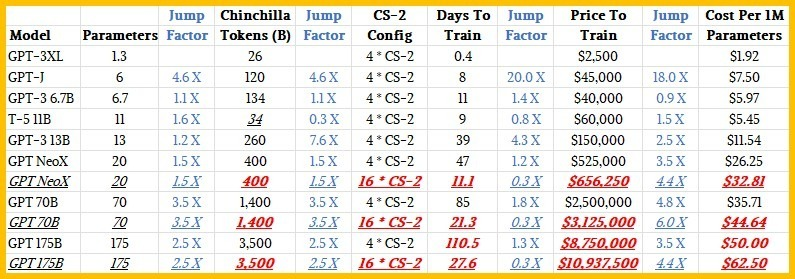
\includegraphics[max height=\textheight,max width=\textwidth]{figures/transformer.jpeg}
	\caption{Transformer}
\end{figure}
% \section{Proposed Model}

\begin{figure}[h!]
	\centering
	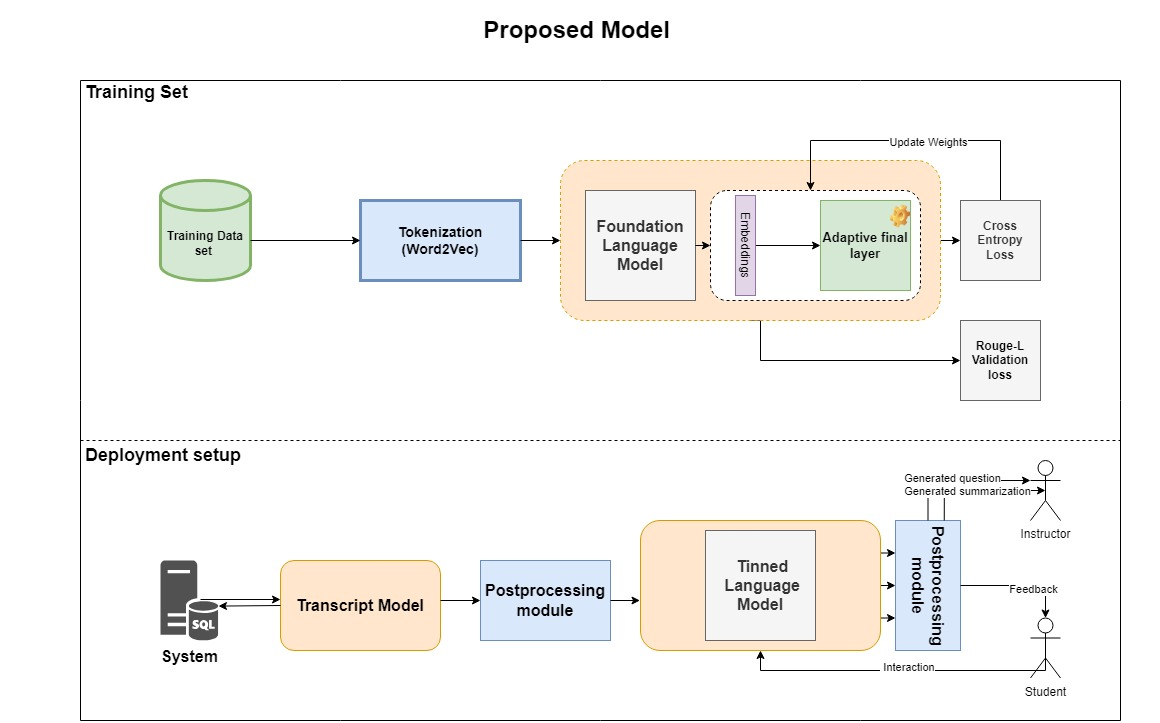
\includegraphics[max height=\textheight,max width=\textwidth]{figures/proposal-model.jpeg}
	\caption{Proposed Model}
\end{figure}

\newpage
\noindent
The motivation behind designing a large language model with adaptive layers lies in the pursuit of creating a model that can efficiently and effectively adapt to the complexities and nuances of different datasets and tasks

\subsection{Flexibility Across Diverse Tasks:}

Adaptive layers enhance the model's flexibility to handle various natural language processing tasks. Whether it's text classification, language translation, sentiment analysis, or any other task, the adaptive layers allow the model to dynamically adjust its parameters based on the specific requirements of each task.

\subsection{Optimizing for Different Data Distributions:}

Different datasets may exhibit varying data distributions and characteristics. Adaptive layers provide a mechanism for the model to adapt its learning rates or normalization parameters dynamically, optimizing its performance for the specific patterns present in the data.



\subsection{Enhanced Convergence and Training Speed:}

Adaptive learning rate methods contribute to faster convergence during training. By adapting learning rates for individual parameters, the model can converge more quickly, leading to reduced training times and improved overall efficiency.
\section{Use Case Analysis}
A Use Case is a type of behavioral representation that shows the interactions
between a system and its users, or actors. It is used to represent and model the
functionality of a system. The main purpose of a use case diagram is to capture
the functional requirements of a system. 
\\ \\ \\
\textbf{There are two formats to represent use cases:}
\begin{enumerate}
    \item Use case diagram.
    \item Use case specifications or scenario in textual format.
\end{enumerate}

\newpage

\section{Use Case Diagram}
\begin{figure}[h!]
	\centering
	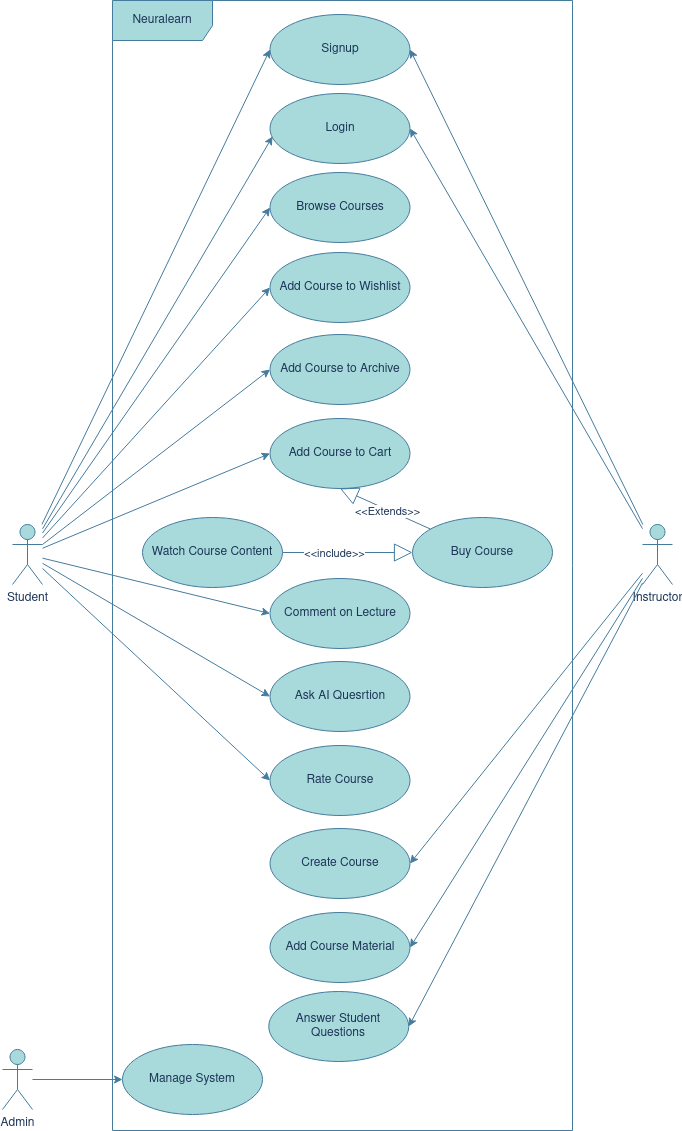
\includegraphics[scale=0.5]{figures/UML-Use-Case.png}
	\caption{UML Use Case Diagram}
\end{figure}

\newpage

\begin{table}[h!]
    \centering
    \caption{Use Case: Sign-Up}
    \bgroup
    \def\arraystretch{1.5}%  1 is the default, change whatever you need
    \begin{tabular}{|m{4cm}|m{11cm}|}
        \hline
        \textbf{Use Case Name} & Sign-Up \\
        \hline
        \textbf{Number} & 1 \\
        \hline
        \textbf{Actor} & Student, Instructor, and Admin \\
        \hline
        \textbf{Preconditions} & 
        \begin{itemize}[noitemsep,topsep=0pt] % Adjust the value as needed
            \item Full name
            \item Email address
            \item Date of birth
            \item Username
            \item Password (and password confirmation)
        \end{itemize} \\
        \hline
        \textbf{Flow of Events} & 
        \begin{itemize}[noitemsep,topsep=0pt]
            \item The student clicks on the sign-up button, leading to the registration form page.
            \item The form prompts the student to enter their full name, email address, date of birth, username, and password.
            \item The student fills in the required information and clicks the "Submit" button.
        \end{itemize} \\
        \hline
        \textbf{Exception} & 
        If the verification email is not received, the student may have the option to request a new verification. \\
        \hline
    \end{tabular}
    \egroup
\end{table}

\newpage

\begin{table}[h!]
    \centering
    \caption{Use Case: Login}
    \bgroup
    \def\arraystretch{1.5}%  1 is the default, change whatever you need
    \begin{tabular}{|m{4cm}|m{11cm}|}
        \hline
        \textbf{Use Case Name} & Login \\
        \hline
        \textbf{Number} & 2 \\
        \hline
        \textbf{Actor} & Student, Instructor, and Admin \\
        \hline
        \textbf{Preconditions} & 
        \begin{itemize}[noitemsep,topsep=0pt] % Adjust the value as needed
            \item The student has successfully registered an account on the platform.
            \item The student has a valid username/email and password.
        \end{itemize} \\
        \hline
        \textbf{Flow of Events} & 
        \begin{itemize}[noitemsep,topsep=0pt]
            \item The student clicks on the sign-up button, leading to the registration form page.
            \item The form prompts the student to enter their full name, email address, date of birth, username, and password.
            \item The student fills in the required information and clicks the "Submit" button.
        \end{itemize} \\
        \hline
        \textbf{Postcondition} & 
        \begin{itemize}[noitemsep,topsep=0pt]
            \item The student is successfully logged into the platform.
            \item The platform displays the student's personalized dashboard with relevant information.
            \item Can Browse Courses
            \item Add Course to wishlist
            \item Add Course to Archive
            \item Add Course to Cart
            \item Comment on lecture
            \item Rate Courses
            \item Ask Question
        \end{itemize} \\
        \hline
        \textbf{Exception} & 
        Invalid Credentials: If the entered credentials are invalid (e.g., incorrect password or username), the platform displays an error message and prompts the student to re-enter the information. \\
        \hline
    \end{tabular}
    \egroup
\end{table}

\newpage

\begin{table}[h!]
    \centering
    \caption{Use Case: Add Course to Cart}
    \bgroup
    \def\arraystretch{1.5}%  1 is the default, change whatever you need
    \begin{tabular}{|m{4cm}|m{11cm}|}
        \hline
        \textbf{Use Case Name} & Add Course to Cart \\
        \hline
        \textbf{Number} & 3 \\
        \hline
        \textbf{Actor} & Student \\
        \hline
        \textbf{Preconditions} & 
        \begin{itemize}[noitemsep,topsep=0pt] % Adjust the value as needed
            \item The student is logged into their account.
            \item The student has navigated to the course catalogue or details page.
        \end{itemize} \\
        \hline
        \textbf{Flow of Events} & 
        \begin{itemize}[noitemsep,topsep=0pt]
            \item The student browses the available courses in the platform's catalogue.
            \item The student selects a course they are interested in by clicking on its title or a designated "Add to Cart" button.
            \item The platform adds the selected course to the student's shopping cart.
            \item Optionally, the student may choose to view their cart to review the selected course and its details.
            \item The student may choose to continue browsing and adding more courses to the cart.
        \end{itemize} \\
        \hline
        \textbf{Postcondition} & 
        The selected course is successfully added to the student's shopping cart. \\
        \hline
        \textbf{Exception} & 
        \begin{itemize}[noitemsep,topsep=0pt]
            \item If the student tries to add a course to the cart that is already present, the platform recognizes this as a duplicate request.
            \item In case of technical issues, such as server downtime or network problems, during the course addition to the cart, the platform informs the student about the problem.
        \end{itemize} \\
        \hline
    \end{tabular}
    \egroup
\end{table}

\newpage

\begin{table}[h!]
    \centering
    \caption{Use Case: Buy Course}
    \bgroup
    \def\arraystretch{1}%  1 is the default, change whatever you need
    \begin{tabular}{|m{4cm}|m{11cm}|}
        \hline
        \textbf{Use Case Name} & Buy Course \\
        \hline
        \textbf{Number} & 4 \\
        \hline
        \textbf{Actor} & Student \\
        \hline
        \textbf{Preconditions} & 
        \begin{itemize}[noitemsep,topsep=0pt] % Adjust the value as needed
            \item The student has added at least one course to their shopping cart.
        \end{itemize} \\
        \hline
        \textbf{Flow of Events} & 
        \begin{itemize}[noitemsep,topsep=0pt]
            \item The student decides to proceed with the purchase.
            \item The student views the contents of their shopping cart, confirming the courses they want to purchase.
            \item The student clicks on the "Proceed to Checkout" button.
            \item The platform prompts the student to provide billing information such as credit card details or select a saved payment method.
            \item The student reviews the order summary, including the selected course(s) and the total cost.
            \item The student confirms the purchase by clicking on the "Confirm Purchase" or "Place Order" button.
            \item The platform processes the payment using the provided billing information.
            \item Successful payment, the platform displays a purchase confirmation message.
        \end{itemize} \\
        \hline
        \textbf{Postcondition} & 
        \begin{itemize}[noitemsep,topsep=0pt]
            \item The purchased course is now accessible in the student's account.
            \item The student may receive a confirmation email with details of the purchase.
        \end{itemize} \\
        \hline
        \textbf{Exception} & 
        \begin{itemize}[noitemsep,topsep=0pt]
            \item If the student attempts to purchase a course but does not have sufficient funds in their account, the platform notifies the student about the insufficient balance.
            \item The student may be prompted to try the purchase again or choose an alternative payment method.
            \item In the event of a technical issue or a failure in processing the payment transaction, the platform informs the student about the problem.
        \end{itemize} \\
        \hline
    \end{tabular}
    \egroup
\end{table}

\newpage

\begin{table}[h!]
    \centering
    \caption{Use Case: Add Course Material}
    \bgroup
    \def\arraystretch{1.5}%  1 is the default, change whatever you need
    \begin{tabular}{|m{4cm}|m{11cm}|}
        \hline
        \textbf{Use Case Name} & Add Course Material \\
        \hline
        \textbf{Number} & 5 \\
        \hline
        \textbf{Actor} & Instructor \\
        \hline
        \textbf{Preconditions} & 
        \begin{itemize}[noitemsep,topsep=0pt] % Adjust the value as needed
            \item The instructive actor is logged into the platform.
            \item The instructive actor has the necessary permissions to add course materials.
            \item A course has been created, and the instructive actor has access to it.
        \end{itemize} \\
        \hline
        \textbf{Flow of Events} & 
        \begin{itemize}[noitemsep,topsep=0pt]
            \item The instructive actor navigates to the course dashboard or management section.
            \item The instructive actor selects the specific course for which they want to add course materials.
            \item Within the course management interface, the instructive actor finds and clicks on the "Materials" or "Content" section.
            \item The instructive actor selects the type of material they want to add and uploads the file or provides the necessary information.
            \item Can use AI to generate Questions or summarization for a section on the course.
        \end{itemize} \\
        \hline
        \textbf{Postcondition} & 
        \begin{itemize}[noitemsep,topsep=0pt]
            \item The course material is successfully added and available within the specified course.
            \item Students enrolled in the course can access the added material based on the visibility settings.
        \end{itemize} \\
        \hline
        \textbf{Exception} & 
        \begin{itemize}[noitemsep,topsep=0pt]
            \item If there is an issue with uploading the material (e.g., file format not supported, network error), the system provides an error message and prompts the instructive actor to try again.
        \end{itemize} \\
        \hline
    \end{tabular}
    \egroup
\end{table}

\newpage

\section{Sequence Diagram}
\begin{figure}[h!]
	\centering
	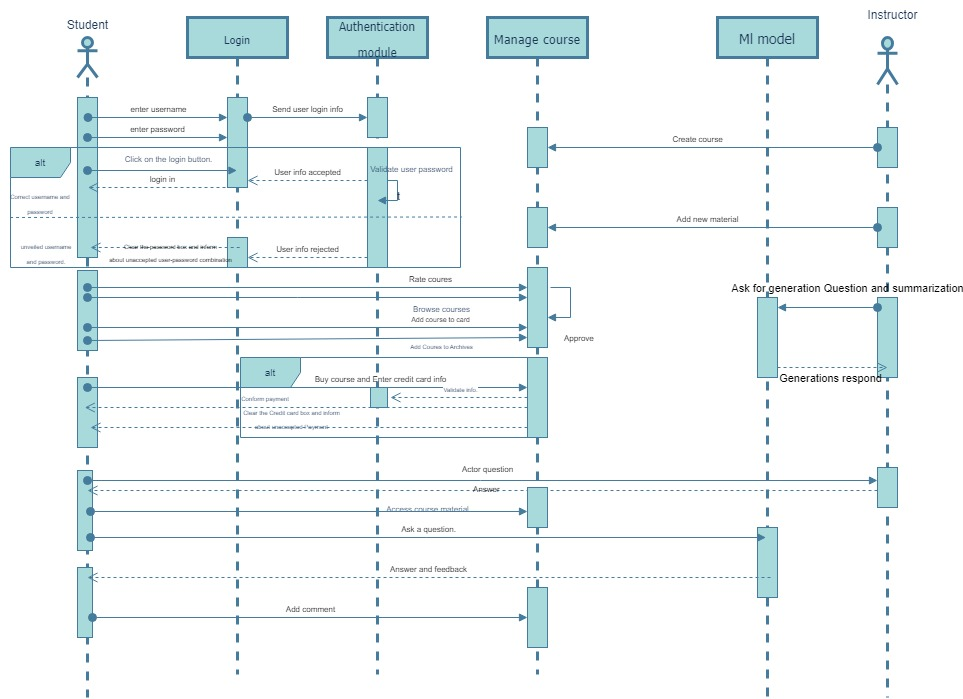
\includegraphics[max height=\textheight,max width=\textwidth]{figures/sequence.jpeg}
	\caption{Sequence Diagram}
\end{figure}

\begin{figure}[h!]
	\centering
	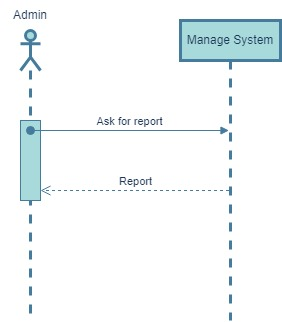
\includegraphics[width=0.40\textwidth]{figures/sequence-admin.jpeg}
	\caption{Sequence Diagram}
\end{figure}

\newpage

\section{Context Diagram}
\begin{figure}[h!]
	\centering
	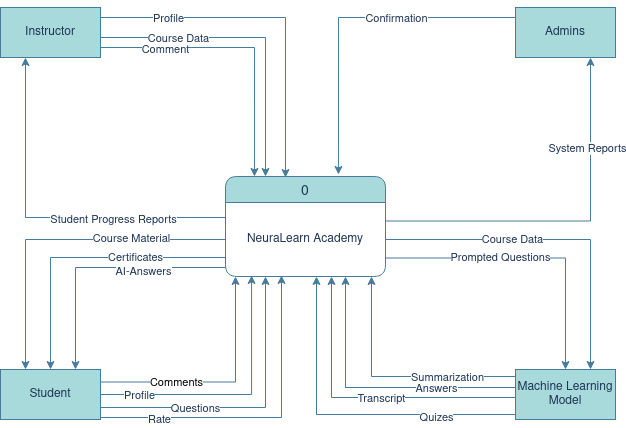
\includegraphics[max height=\textheight,max width=\textwidth]{figures/Context-Diagram.png}
	\caption{Context Diagram}
\end{figure}

\newpage


\section{Data Flow Diagram}
\begin{figure}[h!]
	\centering
	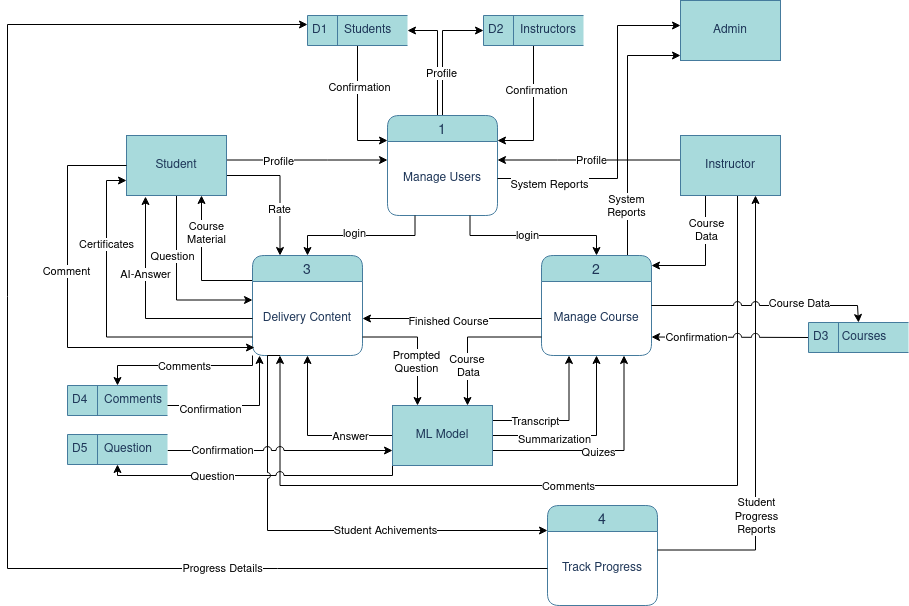
\includegraphics[max height=\textheight,max width=\textwidth]{figures/DFD.png}
	\caption{Data flow Diagram}
\end{figure}

\newpage

\section{Class Diagram}
\begin{figure}[h!]
	\centering
	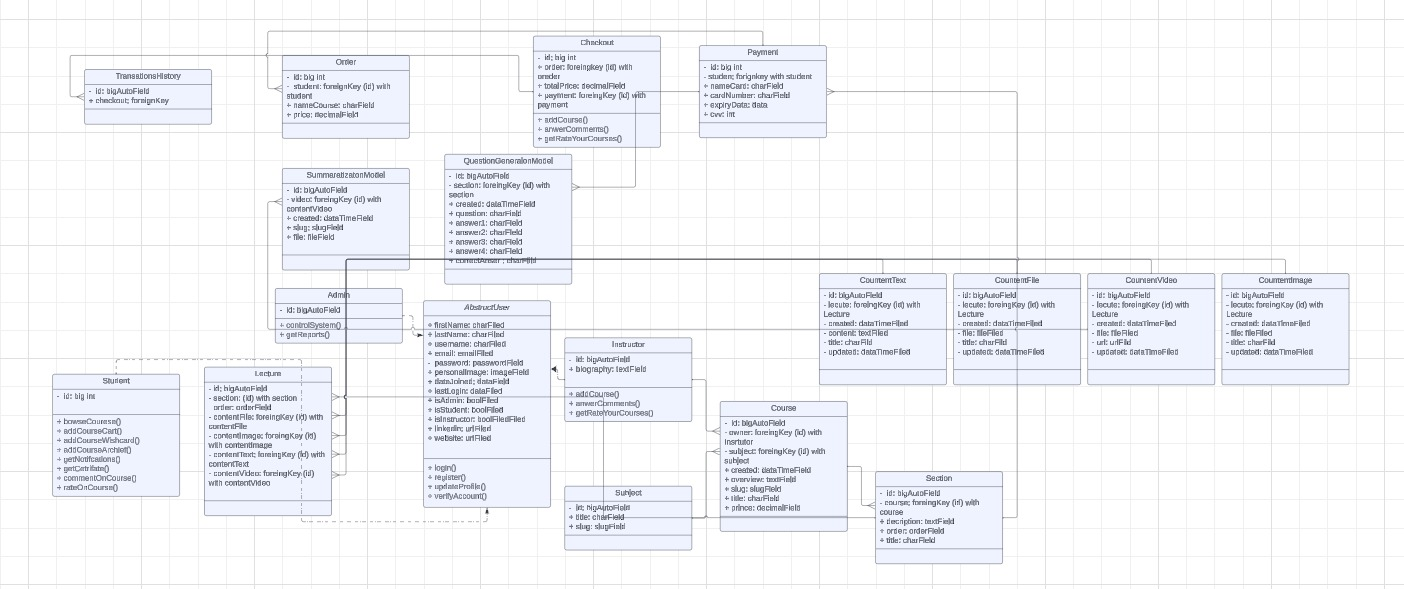
\includegraphics[width=\textwidth]{figures/class-diagram.jpeg}
	\caption{Class Diagram}
\end{figure}

\begin{figure}[h!]
	\centering
	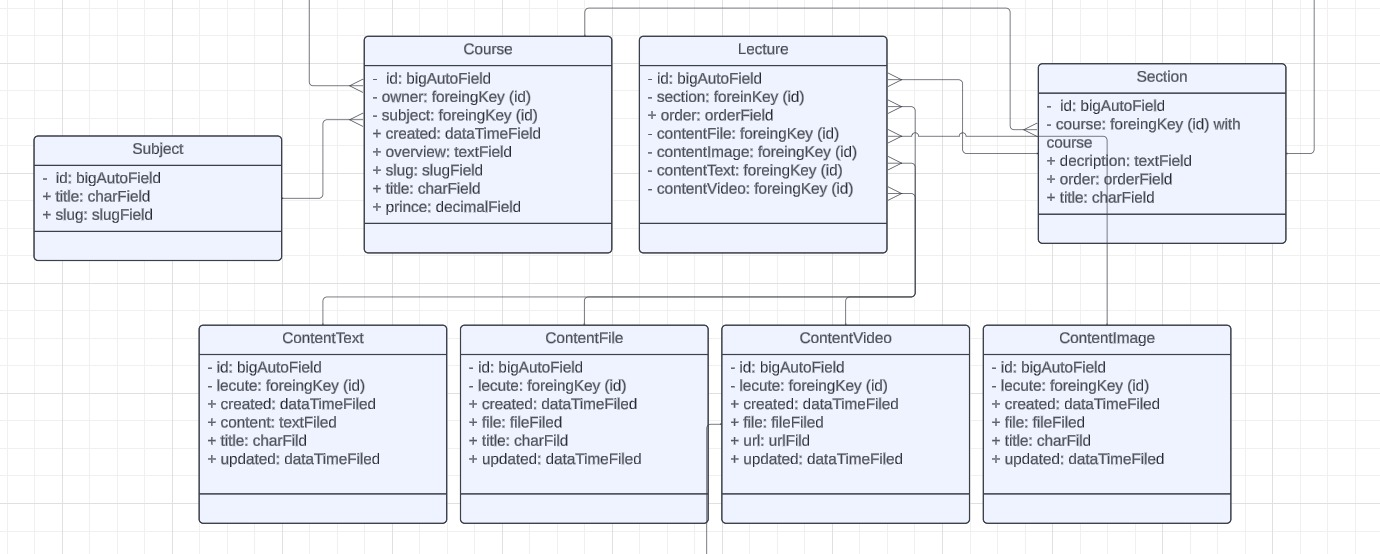
\includegraphics[width=\textwidth]{figures/class-course.jpeg}
	% \caption{Class Diagram}
\end{figure}

\begin{figure}[h!]
	\centering
	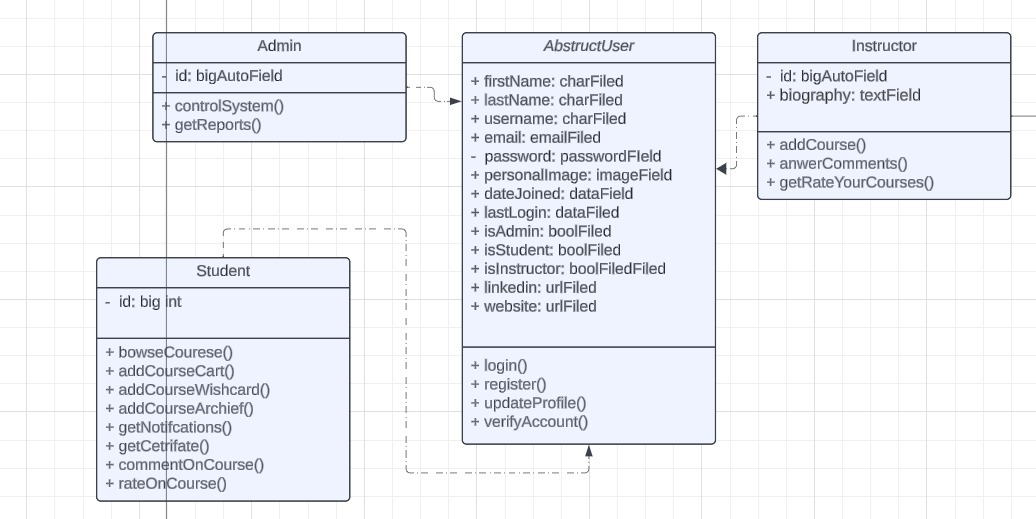
\includegraphics[width=\textwidth]{figures/class-users.jpeg}
	% \caption{Class Diagram}
\end{figure}

\begin{figure}[h!]
	\centering
	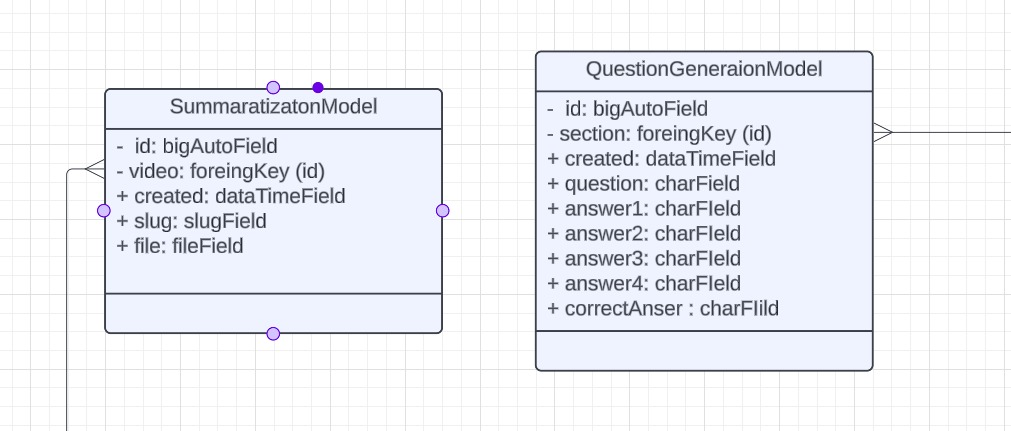
\includegraphics[width=\textwidth]{figures/class-question.jpeg}
	% \caption{Class Diagram}
\end{figure}

\begin{figure}[h!]
	\centering
	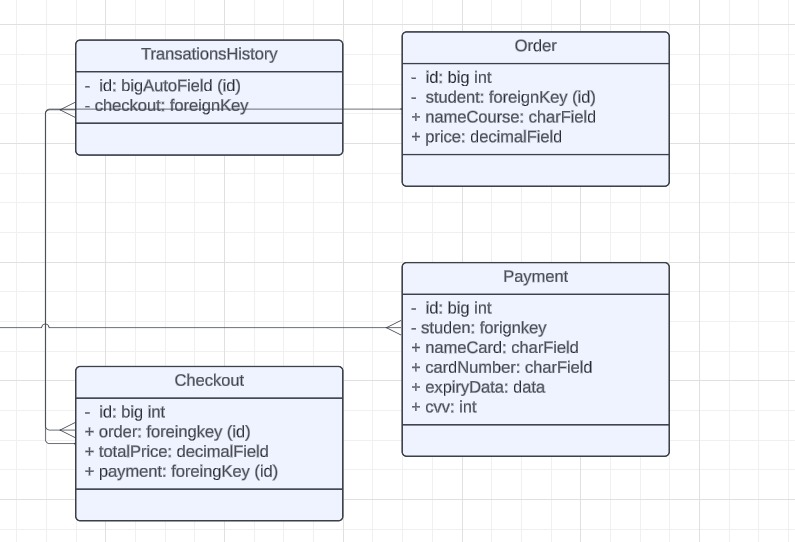
\includegraphics[width=\textwidth]{figures/class-checkout.jpeg}
	% \caption{Class Diagram}
\end{figure}